\section{Implementering}

\subsection{Hostname}
For at udskrive hostnavnet i kommando-prompt'en, har vi åbnet filen "/proc/sys/kernel/Hostname" med fopen. Derefter læser vi første linje i filen ind i en buffer med fgets, og scanner linjen ind i vores hostname variabel med sscan. Til sidst lukker vi filen med fclose. Der er ikke nogen fejlhåndtering hvis filen ikke indeholder noget, eller hvis den ikke eksisterer. Begrundelsen for at vi ikke fejlhåndterer her, er at vi initialiserer vores hostname variabel med strengen "DEFAULT" og derefter overskriver denne variabel, hvis altså filen eksisterer og indeholder tekst. Hvis ikke, bliver variablen ikke overskrevet, og shell'en vil altså udksrive "DEFAULT".

\subsection{Kommando håndtering}
Da vi skulle håndtere kommandoer, syntes det at være nemmere, hvis vi vendte listen af kommandoer om. Mere om dette i afsnit \ref{subsec:pipe_redirect} Piping og redirection

\subsubsection{Valg af exec funktion}
Vi valgte først at afgrænse de mulige exec funktioner til de tre, der understøttede automatisk opslag efter eksekverbare filer i de filkataloger, der er specifiseret i PATH miljøvariabelen. Disse er execlp(), execvp() og execvpe(). Dette gør det let at køre kommandoer som ls og wc.

Funktion en execvpe() blev udelukket, fordi den understøtter ekstra funktionalitet, som vi ikke har brug for i form af muligheden for at specifisere miljøet af filer den eksekverede.

Forskellen på execlp() og execvp() er kun formateringen af argumenterne, og her foretrak vi execvp(), frodi vi har brugt den før.

\subsection{Baggrundskørsel af kommandoer}
Vi har valgt at implementere to forskellige måder at forke på. En "foregroundcmd" og en "backgroundcmd", begge er at finde i forback.c. Foregroundcmd forker, og får forælderprocessen til at vente på at barneprocessen terminerer, mens backgroundcmd forker og derefter returnerer til forælderprocessen, således at barneprocessen blot kører i baggrunden uden at shellen venter på den.

\subsection{Piping og redirection}
\label{subsec:pipe_redirect}
Redirection og piping er blevet implementeret i samme kode, da det stort set er samme funktionalitet.
Der oprettes der en pipe, hver gang en kommando k1 skal sende sit output til k2, oprettes der en pipe hvis skriveende gives som k1's input fil og læse end gives til k2's læseende. Dette kan ses på figur \ref{fig:pipe}. Input- og output redirection kan således ses som en halv pipe, som gives til henholdvis den første og sidste kommando der skal eksekveres. Det sker ved at filerne åbnes i hovedprocessen, og deres filedescriptors kan herefter bruges på samme måde som pipe-ender. Løbende lukker hovedprocessen for filer og pipe-ender, som fremover ikke vil skulle bruges af kommandoer.


\vspace{1cm}
\begin{figure}
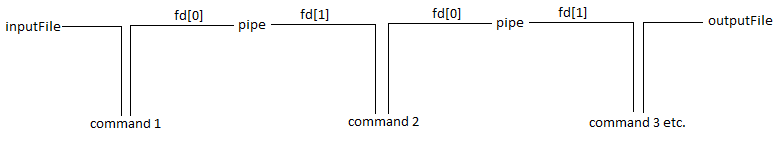
\includegraphics[scale=0.7, trim= 2cm 0cm 0cm 0cm]{pipefig}
\caption{En simpel figur over hvordan der pipes mellem de forskellige kommandoer og in- og output filerne.}
\label{fig:pipe}
\end{figure}

\vspace{1cm}

Vi nåede frem til, at det gav bedst mening at kommandoerne blev udført i den rækkefølge som resultaterne skulle bruges i.
Med andre ord, hvis kommando k1's output skal pipes til kommando k2's input, så skal kommando k1 udføres før kommando k2.
Hovedårsagen til dette valg var, at det gjorde det nemt at køre en kommando-række enten som en række forgrundsprocesser eller baggrundsprocesser, da kommandoerne bare kan udføres sekventielt, uden at bekymre sig om der ventes på en forgrundsproces. For at kunne have samtidig kørsel af kommandoer der undervejs generere output der pipes til hinanden, så køres kun den sidste kommando som forgrundsproces. Det har medført, at hvis den sidste kommando terminere før de forudgående baggrundsprocesser, kan et ske at baggrundsprocesser efterlades kørende, hvilket vi er nået frem til er årsagen til må være årsagen til at listen oprindeligt vendte som den gjorde. Disse baggrundsprocesser er dog ikke synlige for brugeren, men det er muligivis stadigvæk problematisk, hvis en af de efterladte baggrundsprocessor fylder en skrive-enden af en pipe kan der opstå et deadlock, men det må også kunne ske, ved eksekvering i den omvendte rækkefølge.

\subsection{Exit kommando}
Afslutning af bosh programmet sker, når brugeren skriver "exit" i kommandolinjen. I filen bosh.c i metoden executeshellcmd() foregår der et check af kommandoerne. Hvis den første kommando er "exit", så returner executeshellcmd() tallet 1 til den kaldende metode, main metoden. Her bliver terminate sat til 1 og while loopet, der holder bosh kørende ved at chekke om terminate IKKE er 1, vil slutte og derved også bosh.

\subsection{ctrl+c}
Vi fanger ctrl+c gennem kommandoen "signal(SIGINT, interruptRun);". Denne fanger ethvert ctrl+c og, i stedet for at interrupte bosh-kørselen, kaldes "void interruptRun(int dummy)" metoden. interrruptRun udskriver blot "caught ctrl+c" og fortsætter herefter kørslen af programmet. Grunden til at vi ikke sender interruptet videre ned i evt. kørende programmer, er at disse samtidig vil fange det samme ctrl+c input og terminere. Altså er der ikke behov at vi aktivt terminerer dem. Det skal dog også nævnes at dette ikke vil terminere evt. baggrundsprocesser, da disse ikke vil fange ctrl+c inputtet, men da vi har modelleret vores shell efter linux's indbyggede terminal, og denne har samme opførsel, så antager vi at dette er acceptabelt. 

